\documentclass{article}
\IfFileExists{iclr2025_conference.sty}{\usepackage{iclr2025_conference,times}}{
  \usepackage[margin=1in]{geometry}\usepackage{times}
  \usepackage[round,authoryear]{natbib}}
\usepackage[T1]{fontenc}
\usepackage[utf8]{inputenc}
\usepackage{amsmath,amssymb,booktabs,graphicx,microtype,xcolor,enumitem,multirow}
\usepackage{flafter}
\usepackage{tikz}
\usetikzlibrary{arrows.meta,positioning,fit}
\usepackage{hyperref,url}
\definecolor{dynblue}{HTML}{DCEBFA}
\definecolor{physorange}{HTML}{FBE4CB}
\definecolor{datagreen}{HTML}{DDEFD8}
\definecolor{learnpurple}{HTML}{E9DDF2}
\definecolor{projred}{HTML}{F5D4D4}
\newcommand{\done}{\(\boxtimes\)}
\newcommand{\todo}{\(\square\)}
\newcommand{\model}{\textsc{DiffMars}}
\newcommand{\Ls}{L_\mathrm{s}}
\newcommand{\fast}{\textit{Fast strategy:}}
\newcommand{\evidence}{\textit{Evidence:}}

\title{A Differentiable General Circulation Model for Mars:\\
Stable Seasonal Climate and Gradient-Based Physical Calibration}
\author{Anonymous authors}
% \iclrfinalcopy

\begin{document}
\maketitle

\begin{abstract}
Planetary climate models face sparse observations, unfamiliar regimes, and
stringent physical constraints. We develop \model, a modular differentiable
general circulation model (GCM) for Mars with explicit, auditable physics. A JAX spectral
primitive-equation core is coupled to eccentric-orbit and diurnal forcing,
correlated-\(k\) carbon-dioxide radiation, prescribed dust, MOLA topography, TES
surface properties, multilayer regolith, boundary-layer mixing, dry convection,
and a surface \(\mathrm{CO_2}\) cycle. A global projection reconciles the
log-pressure dynamical variable with atmosphere--frost mass exchange. At T21/12
levels and a 300\,s timestep, a clean 668-sol integration remains finite and
limits relative atmosphere-plus-frost \(\mathrm{CO_2}\) drift to
\(1.22\times10^{-9}\). Surface pressure correlates with MOLA elevation at
\(-0.960\). A season-matched diagnostic against ARCO-MACDA gives pressure and
temperature spatial correlations of 0.987 and 0.953, while exposing weak wind
agreement and a \(+13.4\) K warm bias. Automatic differentiation of an
eight-step rollout agrees with centered finite differences to
\(6.1\times10^{-10}\) relative error. On an 11-core Apple M3 Pro, the
steady-state invocation advances 107.9 simulated sols per wall hour. These
results establish a stable, differentiable physical baseline and a versioned
reanalysis comparison pipeline. The model contains no neural component; its
differentiability is used to diagnose and calibrate interpretable physical
parameters.
\end{abstract}

\section{Introduction}

Mars is a useful and unusually strict test of hybrid climate modeling. Its thin,
mostly \(\mathrm{CO_2}\) atmosphere is coupled to large relief, strong seasonal
and diurnal forcing, and heterogeneous surface properties. In winter, a material
fraction of the atmosphere condenses onto the polar surface and returns in
spring \citep{leighton1966co2,guo2009seasonal}. Airborne dust both attenuates
sunlight and heats the atmosphere, changing thermal tides and the global
circulation \citep{madeleine2011dust,montabone2015dust}. Low atmospheric heat
capacity couples those effects tightly to regolith heat storage and boundary-layer
mixing. A model can therefore match one field for the wrong reason: excess
infrared opacity can offset weak soil storage, while excess drag can hide an
incorrect vertical heating profile.

The observing system makes such compensating errors difficult to identify.
MOLA and TES constrain topography and surface properties
\citep{smith2001mola,christensen2001tes}, while landers such as InSight provide
high-frequency local weather \citep{banfield2020insight}. There is no uniformly
observed global atmospheric state. Mars Climate Sounder profiles constrain
temperature, water vapor, dust, condensates, and polar energy balance
\citep{mccleese2007mcs}. MACDA, EMARS, and OpenMARS assimilate
spacecraft retrievals into different Mars GCMs
\citep{montabone2014macda,greybush2019emars,holmes2020openmars}. These products
are indispensable references, but they retain model and assimilation assumptions.

Mature physical Mars GCMs encode decades of knowledge. PlanetWRF spans local to
global planetary circulation \citep{richardson2007planetwrf}; the LMD planetary
climate model and NASA Ames GCM include vertically resolved radiation, dust, surface
thermodynamics, turbulent mixing, and volatile cycles
\citep{forget1999improved,haberle2019ames}. Their computational cost grows with
resolution, and resolution itself changes wave--mean-flow interactions
\citep{kling2025resolution}. A new model must consequently demonstrate more than
low snapshot error: it must show stability, closed budgets, seasonal phase and
amplitude, vertical structure, and measured computational cost.

NeuralGCM provides the architectural precedent. It combines a differentiable
spectral core with learned physical tendencies and trains the coupled model end
to end \citep{kochkov2024neuralgcm}. Stable learned closures require prognostic,
not merely one-step, validation \citep{yuval2020stable}. Fully differentiable
intermediate-complexity models likewise support parameter inference and coupled
optimization \citep{davenport2026jcm}. Recent Mars foundation models instead
learn fast global forecasts directly from reanalysis
\citep{roy2026foundation,singh2026aircast}. Our complementary goal is an
auditable physics-first simulator whose learned component is narrow, whose
reservoirs remain explicit, and whose errors can be traced to processes.

This distinction matters for planetary experiments. A hybrid GCM can expose
derivatives with respect to physical parameters or forcing, but only if those
derivatives pass through a stable, meaningful climate model. The longer-term
motivation includes controlled planetary-climate experiments. Although warming
proposals have a long history \citep{sagan1973planetary,mckay1991making},
accessible Martian \(\mathrm{CO_2}\) cannot produce an Earth-like climate
\citep{jakosky2018inventory}. Present-day validation is therefore a prerequisite;
recent calls for terraforming research do not remove that validation requirement
\citep{debenedictis2025case}. This paper makes no terraforming-outcome claim.

The question at this snapshot is narrower: can a compact differentiable Mars GCM
survive a complete seasonal cycle while preserving the dominant mass budget and
exposing identifiable physical errors? We answer with a hierarchy of evidence.
Core tests establish implementation correctness; a complete Mars-year rollout
tests stability and conservation; MOLA, ARCO-MACDA, Ames, and MCD provide
complementary structural and climatic diagnostics; and measured throughput
establishes the cost of producing those results.

Our completed contributions are: (i) a planet-parameterized Mars GCM built on the
Dinosaur spectral core \citep{dinosaur2024}; (ii) explicit orbit,
multiband radiation, dust, surface, regolith, boundary-layer, convection, and
seasonal-cap operators connected by a typed tendency interface; (iii) an
atmosphere--surface \(\mathrm{CO_2}\) projection and scale-selective diffusion
that permit a clean 668-sol integration; (iv) a versioned ARCO-MACDA pipeline
with a leakage-safe Mars-year split; and (v) executable evidence for gradients,
mass conservation, topographic structure, reference error, failure diagnosis,
and runtime; and (vi) a bounded gradient-based calibration interface for the
CO$_2$ opacity, dust opacity, and surface-exchange strength.

\section{Background and Related Work}

\subsection{Mars models and reference products}
PlanetWRF provides a general local-to-global dynamical framework
\citep{richardson2007planetwrf}. The LMD model established a comprehensive
framework extending above 80 km \citep{forget1999improved}; NASA Ames supplies
an independently developed reference \citep{haberle2019ames}. MCD v6.1 exposes LMD simulations through
season-, location-, altitude-, local-time-, and dust-matched queries
\citep{mcd61}. We treat Ames and MCD as model references, never observational
truth. MOLA and TES are static boundary inputs. MACDA, EMARS, and OpenMARS are
data-assimilating products, and comparing them reveals sensitivity to the parent
model and assimilation system. ARCO-Mars republishes all three as cloud-optimized
archives, allowing bounded reads instead of full downloads
\citep{bhattacharya2026arcomars}.

The reference roles are intentionally separate. ARCO-MACDA supplies consecutive
global states and supplies targets for physical-parameter calibration and
diagnosis. Held-out MACDA years measure temporal transfer; ARCO-EMARS and
ARCO-OpenMARS measure
reference dependence. Ames and MCD provide model-family comparisons, and local
lander data can provide a direct observational anchor. No product serves at once
as boundary condition, calibration target, and sole diagnostic reference.

\subsection{Surrogates, recurrent models, and intervention use}
Fast emulation of an expensive Mars GCM is already possible in restricted
settings. \citet{tunnell2023gp} trained a Gaussian-process emulator of NASA Ames
GCM sensitivity experiments, reducing selected predictions from weeks of model
computation to minutes. This is strong evidence that parameter ensembles can be
accelerated, but such a surrogate maps within a designed parameter domain and is
not automatically a recurrent global-state simulator. Reliability under large,
sequential interventions still depends on training coverage and uncertainty.

World models instead learn a recurrent latent transition used for prediction or
planning \citep{ha2018worldmodels}. Terraforming would eventually require this
action-conditioned view because one intervention changes the state on which the
next action operates. Our present contribution stops earlier: \model{} supplies
an explicit, differentiable transition and constrained reservoirs, but has no
latent planner or policy. This boundary keeps the paper testable. A future
surrogate can be judged against a verified physical transition rather than being
asked simultaneously to discover Mars dynamics, enforce conservation, and plan.

\subsection{Coupled Mars processes}
Orbital geometry and surface properties set solar heating; regolith storage and
turbulent exchange determine its diurnal and seasonal response. Dust adds solar
scattering and absorption as well as infrared opacity
\citep{madeleine2011dust}. Because gaseous absorption varies with wavelength,
pressure, and temperature, two-stream and correlated-\(k\) methods compress a
costly spectral transfer problem \citep{toon1989twostream}. The vertical heating
profile matters as much as the surface mean because winds respond to horizontal
and vertical temperature gradients. At the polar caps, condensation couples
latent heat, surface optics, atmospheric mass, and circulation. These links
motivate explicit process operators, budget tests, and bounded physical calibration.

\subsection{Differentiable and hybrid GCMs}
NeuralGCM combines spectral primitive-equation dynamics with learned
parameterizations \citep{kochkov2024neuralgcm}; JCM shows that an
intermediate-complexity atmosphere can be fully differentiable
\citep{davenport2026jcm}. \model{} adopts the same computational advantages---a
JAX-native spectral core and differentiable coupled rollout---while keeping all
reported tendencies deterministic. Differentiation is used for parameter
inference rather than for training a neural closure.

\subsection{Verification before learning}
Parameter tuning can hide a numerical defect while reducing loss. We therefore use
standard spherical and atmospheric-core tests
\citep{williamson1992standard,held1994proposal,jablonowski2006baroclinic}, then
measure column-energy closure, surface exchange, frost positivity, total
\(\mathrm{CO_2}\), topographic pressure, and seasonal stability.

A strong eventual result needs five types of evidence: numerical correctness;
mass, energy, and angular-momentum integrity; season- and local-time-matched
climatological fidelity; withheld-year and dust-storm generalization; and utility
measured by wall time, memory, and stability beyond the calibration horizon. The
present results fully establish the first category and part of the next two.

\section{Method}

\subsection{Differentiable physical formulation}
Let \(x_t\) contain spectral vorticity, divergence, temperature variation,
log-surface-pressure, and time, and let \(s_t\) contain surface temperature,
\(\mathrm{CO_2}\)-ice pressure equivalent, and soil temperatures:
\begin{equation}
\frac{d}{dt}\begin{bmatrix}x\\s\end{bmatrix}
=\mathcal D_\theta(x;b)+\mathcal P_\phi(x,s,b,t).
\label{eq:hybrid}
\end{equation}
\(\mathcal D_\theta\) is resolved dynamics and \(\mathcal P_\phi\) is
deterministic column physics. The calibrated subset of \(\phi\) contains the
CO$_2$ and dust longwave-opacity scales and a bulk surface-exchange multiplier.

\begin{figure}[t]
\centering
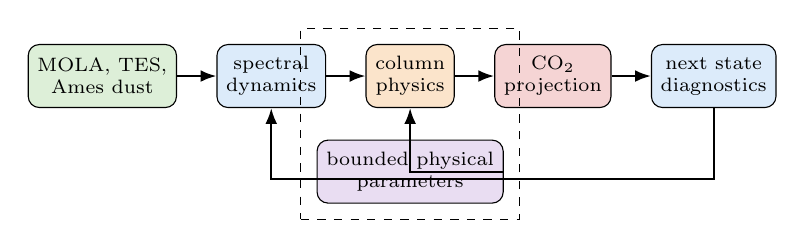
\begin{tikzpicture}[node distance=4mm and 5mm,
 box/.style={draw,rounded corners,align=center,minimum height=8mm,font=\scriptsize},
 arr/.style={-{Latex[length=2mm]},thick}]
\node[box,fill=datagreen] (data) {MOLA, TES,\\Ames dust};
\node[box,fill=dynblue,right=of data] (dyn) {spectral\\dynamics};
\node[box,fill=physorange,right=of dyn] (phys) {column\\physics};
\node[box,fill=learnpurple,below=of phys] (learn) {bounded physical\\parameters};
\node[box,fill=projred,right=of phys] (proj) {CO\(_2\)\\projection};
\node[box,fill=dynblue,right=of proj] (out) {next state\\diagnostics};
\draw[arr] (data)--(dyn);\draw[arr] (dyn)--(phys);\draw[arr] (phys)--(proj);
\draw[arr] (learn.east)-|(phys.south);\draw[arr] (proj)--(out);
\draw[arr] (out.south)|-++(0,-9mm)-|(dyn.south);
\node[draw,dashed,fit=(phys)(learn),inner sep=2mm] {};
\end{tikzpicture}
\caption{\model{} couples spectral dynamics to deterministic Mars physics.
Automatic differentiation connects diagnostics to bounded physical parameters.}
\label{fig:architecture}
\end{figure}

\subsection{Software framework and execution path}
The implementation separates reusable numerics from Mars configuration. The
\texttt{framework/gcm} package defines coordinates, nondimensionalization,
Dinosaur adapters, IMEX integration, restarts, and benchmarks. The framework
physics module contains JAX-pure column operators and their typed tendency
contract. The Mars package owns
planetary constants, orbit, MOLA/TES staging, Ames dust, and run assembly.
Scripts add chunked execution, checkpoint diagnostics, reference staging, and
evaluation. This dependency direction prevents generic physics from silently
importing Mars constants.

Each physics evaluation transforms spectral fields once to nodal temperature,
wind, and pressure, then shares those arrays among radiation, surface exchange,
drag, PBL diffusion, convection, regolith conduction, and \(\mathrm{CO_2}\)
exchange. Radiation uses fixed-size \texttt{lax.scan} recurrences; vertical
diffusion uses a batched tridiagonal Thomas solve; and convection uses a
fixed-shape weighted pool-adjacent-violators scan. These choices keep compiled
timesteps free of data-dependent Python control flow and make the major column
kernels scale linearly with layer count.

\begin{table}[t]\centering\small
\caption{Implemented software layers.}\label{tab:framework}
\begin{tabular}{p{0.25\linewidth}p{0.67\linewidth}}\toprule
Layer & Responsibility\\\midrule
Dinosaur adapter & Spectral transforms, sigma coordinates, primitive equations,
IMEX step, hyperdiffusion\\
Column physics & Radiation, fluxes, drag, PBL, convection, soil, volatile cycle\\
Mars assembly & Constants, orbit, MOLA/TES, dust, balanced initialization\\
Run/evaluation & JIT rollout, restart, budgets, NetCDF, ARCO/Ames/MCD matching\\\bottomrule
\end{tabular}
\end{table}

\subsection{Resolved dynamics and numerical integration}
The Dinosaur/JAX core \citep{dinosaur2024,jax2018} solves the hydrostatic
primitive equations in terrain-following \(\sigma=p/p_s\) coordinates. In
schematic vector form,
\begin{align}
\frac{D\mathbf v}{Dt}+f\mathbf k\!\times\!\mathbf v
 &= -\nabla_\sigma\Phi-RT\nabla_\sigma\log p_s+\mathbf F_{\rm phys},\\
\frac{DT}{Dt}-\kappa T\frac{D\log p}{Dt}&=Q_{\rm phys},\\
\frac{\partial\log p_s}{\partial t}
 &= -\frac{1}{p_s}\nabla\!\cdot\int_0^1p_s\mathbf v\,d\sigma+S_{\rm CO_2}.
\end{align}
Hydrostatic geopotential follows from \(\partial\Phi/\partial\log p=-RT\).
Vorticity and divergence avoid polar vector singularities. The core resolves
transport, pressure gradients, rotation, and gravity waves; column physics
supplies momentum, heat, and volatile sources.

Production uses T21 (a \(32\times64\) Gaussian nodal grid), 12 sigma layers, a
300\,s semi-implicit timestep, and fourth-order spectral diffusion with a
0.1-sol shortest-mode e-folding time. Diffusion acts only on modal atmospheric
fields, leaving nodal surface, frost, and soil reservoirs unchanged.

\subsection{Orbit, radiation, and dust}
Kepler's equation determines heliocentric distance, true anomaly, \(\Ls\), and
declination. Rotation and longitude determine local hour angle. The corrected
configuration resolves the diurnal zenith angle and slant optical path; the
completed baseline used daily-mean sunlight and is labeled accordingly.

Radiation uses seven solar and five thermal Ames bands, with 16 absorbing
correlated-\(k\) channels and one clear channel per band. Coefficients are
interpolated in temperature and log pressure. A two-stream recurrence propagates
upward and downward fluxes \citep{toon1989twostream}. Prescribed visible and
infrared dust opacity is distributed vertically with an Ames/Conrath profile and
band-dependent scattering and absorption. It represents the leading radiative
effect of dust but not lifting, transport, settling, or particle evolution
\citep{madeleine2011dust}.

Layer heating is computed from flux convergence,
\begin{equation}
Q_k=\frac{g}{c_p\Delta p_k}\left[(F^\downarrow-F^\uparrow)_{k+1/2}
-(F^\downarrow-F^\uparrow)_{k-1/2}\right].
\end{equation}
This closes the discrete column energy budget, although direct Ames-column flux
regression is still needed to validate the opacity calibration.

\subsection{Surface, regolith, PBL, and convection}
Prognostic surface temperature obeys
\begin{equation}
C_s\frac{dT_s}{dt}=F^\downarrow_{\rm SW}-F^\uparrow_{\rm SW}
+F^\downarrow_{\rm LW}-\epsilon\sigma T_s^4-H-G-L_{\rm CO_2}\dot m,
\end{equation}
where \(H\) transfers sensible heat to the atmosphere, \(G\) enters the soil,
and \(\dot m\) is positive for condensation. TES supplies spatial albedo and
thermal inertia. Twelve finite-volume soil layers extend from fractions of the
diurnal skin depth to beyond the annual skin depth; internal conductive fluxes
cancel pairwise and soil state is checkpointed.

Log-law surface stress and sensible exchange are modified by bulk Richardson
stability. An implicit tridiagonal solve mixes heat, momentum, and tracers in the
PBL while conserving the appropriate column integral. Dry adjustment identifies
contiguous unstable blocks and conserves sigma-mass-weighted enthalpy. These
closures capture minimum constraints but remain simpler than mature plume and
Mellor--Yamada-style Mars schemes
\citep{forget1999improved,haberle2019ames,colaitis2013pbl}.

\subsection{Seasonal \texorpdfstring{\(\mathrm{CO_2}\)}{CO2} cycle}
Surface \(\mathrm{CO_2}\) condenses or sublimes from the non-latent energy
residual at a pressure-dependent frost point,
\begin{equation}
T_f(p_s)=\frac{3182.48}{23.3494-\log(p_s/100\,{\rm Pa})}.
\end{equation}
Supply and ice gates prevent removing unavailable mass; latent heat returns to
the surface budget. Atmospheric condensation, frost-dependent optics, and
\(\mathrm{CO_2}\) clouds remain absent.

Because the dycore advances \(\log p_s\), a finite step does not exactly preserve
the linear inventory conserved by the tendency. After each step, negative frost
is repaired and a global pressure scale \(\alpha\) satisfies
\begin{equation}
\int_A(\alpha p_s^*+p_{\rm ice}^*)\,dA
=\int_A(p_s+p_{\rm ice})\,dA-\Delta M_{\rm escape}g.
\end{equation}
Gaussian quadrature evaluates the integrals. The projection preserves the
resolved pressure pattern, maintains positive pressure, and retains an explicit
escape sink when configured.

\subsection{Data, splits, and metrics}
MOLA and TES are boundary inputs, not evaluation targets. ARCO-MACDA has 96,480
states, 35 sigma levels, a \(36\times72\) grid, and exactly 12 samples per sol.
Its logical size is approximately 216 GB, but Zarr permits bounded reads. We
binary-search explicit Mars-year labels, stream native chunks, aggregate daily,
interpolate to 12 levels, periodically regrid to T21, validate finite values,
and record provenance and hashes. The verified ten-sol MY24 atmosphere and
radiation samples test this pipeline; they are not held-out results.

The frozen calibration protocol uses MY32 seasonal windows for fitting, MY33
for stopping and validation, and MY34--35 for final diagnostics; the partial
MY36 tail is excluded. Current MY24 data validate preprocessing only. Metrics use Gaussian
area weights. Relative MAE divides by area-weighted mean absolute reference
magnitude, remaining meaningful for signed winds with near-zero global means.
Explicitly,
\begin{equation}
\mathrm{relative\ MAE}=\frac{\sum_iw_i|y_i-r_i|}{\sum_iw_i|r_i|}.
\end{equation}
Seasonal comparisons must match \(\Ls\), averaging window, local time, vertical
coordinate, dust scenario, and boundary fields. Unmatched comparisons are
labeled diagnostic. We also record checkpoint extrema, volatile drift,
atmospheric energy and angular momentum, post-JIT throughput, and memory.

\begin{figure}[t]
\centering
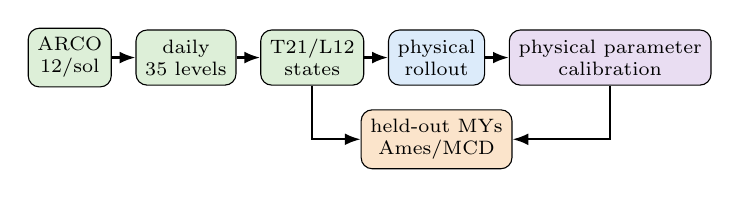
\begin{tikzpicture}[node distance=3mm,
 box/.style={draw,rounded corners,align=center,font=\scriptsize,minimum height=7mm},
 arr/.style={-{Latex[length=2mm]},thick}]
\node[box,fill=datagreen] (a) {ARCO\\12/sol};
\node[box,fill=datagreen,right=of a] (b) {daily\\35 levels};
\node[box,fill=datagreen,right=of b] (c) {T21/L12\\states};
\node[box,fill=dynblue,right=of c] (d) {physical\\rollout};
\node[box,fill=learnpurple,right=of d] (e) {physical parameter\\calibration};
\node[box,fill=physorange,below=of d] (f) {held-out MYs\\Ames/MCD};
\draw[arr](a)--(b);\draw[arr](b)--(c);\draw[arr](c)--(d);
\draw[arr](d)--(e);\draw[arr](e.south)|-(f.east);\draw[arr](c.south)|-(f.west);
\end{tikzpicture}
\caption{Reanalysis staging, physical calibration, and held-out diagnostic flow.}
\label{fig:data}
\end{figure}

\begin{table}[t]
\centering\small
\caption{Completed physical-baseline configuration.}\label{tab:config}
\begin{tabular}{ll}\toprule
Component & Choice\\\midrule
Grid/time & T21, \(32\times64\), 12 sigma levels, 300\,s\\
Boundary & MOLA; TES albedo and thermal inertia\\
Forcing & eccentric orbit; daily mean in completed run\\
Radiation & Ames correlated-\(k\) CO\(_2\); prescribed dust\\
Surface & prognostic skin, 12 soil layers, CO\(_2\) frost\\
Mixing & Richardson exchange, implicit PBL, dry adjustment\\
Dissipation & fourth order; 0.1-sol shortest-wave time\\\bottomrule
\end{tabular}
\end{table}

\subsection{Method checklist and shortest completion path}
\begin{itemize}[leftmargin=1.8em,itemsep=5pt]
\item[\done] \textbf{Planet-independent dynamics, restarts, and diagnostics.}
\evidence{} Canonical core tests and restart equivalence exercise the framework;
checkpoints retain atmosphere, surface, frost, and soil state.

\item[\done] \textbf{Mars orbit, radiation, dust, surface, regolith, PBL,
convection, and \(\mathrm{CO_2}\).} \evidence{} Every operator has an isolated
conservation or response test and the assembled path completed one Mars year.

\item[\done] \textbf{Inventory projection, diffusion, and ARCO contract.}
\evidence{} The full-year run and hashed ten-sol artifacts exercise these paths;
the Mars-year split is recorded in the dataset contract.

\item[\done] \textbf{Expose bounded physical calibration controls.}
\evidence{} CO$_2$ longwave opacity, dust longwave opacity, and bulk
surface-exchange strength are positive bounded scalars inside the deterministic
physics path. Their JAX gradients pass through radiation, dynamics, diffusion,
and the CO$_2$ projection.

\item[\done] \textbf{Export a common full-state comparison schema.}
\evidence{} Seasonal checkpoints retain all 12 temperature and wind levels,
surface pressure and temperature, frost, soil state, \(L_s\), and local solar
time. ARCO, Ames, and MCD adapters record their averaging and interpolation.

\item[\todo] \textbf{Complete physical calibration.}
The nominal MY34--35, Ames, and MCD diagnostics are complete. Fit the three
parameters on MY32, choose stopping on MY33, and compare L-BFGS with an
equal-budget bounded Powell search before evaluating the fixed calibration.
\end{itemize}

\section{Results}

\subsection{Claim boundary and evidence hierarchy}
The current results ask whether the implementation reproduces known numerical
behavior, survives one seasonal cycle, preserves the dominant volatile
inventory, and exposes identifiable physical errors. This ordering prevents a
high map correlation from being mistaken for a correct climate. The strongest
eventual climate claim also requires repeated-year convergence, season-matched
reference diagnostics, budget preservation, and a measured calibration-cost
tradeoff.

\subsection{Verification and differentiability}
The focused GCM suite passed 127 tests with three skipped, including slow
core benchmarks; the full non-slow package suite passed 292 with three skipped
and five deselected long tests. After the latest changes, 59 directly affected
physics/maps/submission tests pass. These verify contracts, not climate accuracy.

For a T21/four-level eight-step rollout, the derivative of area-mean surface
temperature with respect to uniform albedo is \(-1.0341944645\) K per unit
albedo. Centered finite differences at \(10^{-3}\) and \(10^{-4}\) agree to
relative errors \(6.1\times10^{-10}\) and \(3.5\times10^{-9}\). This establishes
local differentiation through a smooth path, not useful seasonal gradients
across physical switches.

\begin{table}[t]\centering\small
\caption{Numerical evidence at this manuscript snapshot.}\label{tab:num}
\begin{tabular}{lll}\toprule
Check & Result & Scope\\\midrule
Autodiff vs finite difference & \(6.1\times10^{-10}\) & short smooth path\\
Completed integration & 668.0004 sols & finite first year\\
Maximum CO\(_2\) relative drift & \(1.22\times10^{-9}\) & projection effective\\
Pressure--elevation correlation & \(-0.960459\) & topographic structure\\
Final maximum 3-D wind & 129.729 m\,s\(^{-1}\) & finite upper level\\\bottomrule
\end{tabular}
\end{table}

\subsection{Failure diagnosis and stable baseline}
The first unfiltered attempt remained finite through sol 512.166 but reached
2953 m\,s\(^{-1}\) winds and then failed. Total \(\mathrm{CO_2}\) remained
conserved, separating the failure from volatile exchange. Fourth-order diffusion
reduced maximum wind to 46.0 m\,s\(^{-1}\) within 3.332 sols from the degraded
restart. We rejected that recovery and reran from initialization.

The clean run completed 197,673 steps (668.0004 sols); all exported values and
135 checkpoints are finite. Final surface pressure spans 221.82--1078.76 Pa,
temperature 144.33--241.22 K, and near-surface wind 0.20--30.02 m\,s\(^{-1}\).
Atmosphere-plus-frost \(\mathrm{CO_2}\) changed from
\(2.5984358236\times10^{16}\) to \(2.5984358204\times10^{16}\) kg, a relative
drift of \(-1.22\times10^{-9}\). This establishes numerical stability for one
Mars year, not equilibrium.

\subsection{Topography and ARCO-MACDA diagnostic}
T21 MOLA elevation ranges from \(-7.261\) to 14.478 km. Final pressure correlates
with elevation at \(-0.960459\), with a fitted 10.95 km log-pressure scale
height. This confirms boundary alignment and hydrostatic structure but is not an
independent target because MOLA initializes the lower boundary. We compare the
instantaneous state at \(\Ls=359.683^\circ\) to the MY24
ARCO daily mean at \(0.278^\circ\), a \(0.595^\circ\) offset. Pressure and broad
temperature structure agree; winds do not (Table~\ref{tab:arco}). The model is
13.40 K too warm, vector-wind correlations are 0.36--0.47, and frost relative
MAE is 42.9\%. Temporal mismatch and reanalysis ancestry make this diagnostic
rather than held-out validation.

\begin{table}[t]\centering\small
\caption{Compact area-weighted model--ARCO diagnostic. Full metrics appear in
Appendix~\ref{app:fullmetrics}.}\label{tab:arco}
\begin{tabular}{lrrr}\toprule
Field & Bias & MAE & Corr.\\\midrule
Pressure (Pa) & \(-14.12\)&23.57&0.987\\
Surface \(T\) (K) & \(+13.40\)&13.40&0.953\\
East wind (m\,s\(^{-1}\)) & \(-1.16\)&5.48&0.469\\
North wind (m\,s\(^{-1}\)) & \(-1.38\)&5.46&0.361\\
Wind speed (m\,s\(^{-1}\)) & \(+3.45\)&4.71&0.455\\
CO\(_2\) frost (Pa-eq.) & \(-47.33\)&54.74&0.888\\\bottomrule
\end{tabular}
\end{table}

\begin{figure}[t]\centering
\includegraphics[width=\linewidth]{../../outputs/branch_physical_baseline_t21_l12_dt300_hyperdiff01/evaluation/mola_topography_pressure.png}
\caption{MOLA topography and final pressure versus elevation. This tests
boundary alignment and hydrostatic structure, not forecast skill.}\label{fig:mola}
\end{figure}

\subsection{Radiative-bias probes and corrected run}
The \(+13.4\) K bias motivated a process-level energy diagnosis. Daily-mean
sunlight suppresses the large Martian day--night cycle; because emission scales
as \(T^4\), that changes the mean energy balance. The original correlated-\(k\)
path also omitted the zenith-angle air-mass factor and did not use the separately
prescribed infrared dust field. These are identifiable physics-path errors that
parameter tuning should not conceal. Enabling resolved local time, slant paths, and
infrared dust in a ten-sol probe from the year-one restart
reduced matched Ames temperature bias to \(+6.93\) K (MAE 7.05 K, correlation
0.9716). Scaling CO\(_2\) and dust longwave opacity to 0.25 reduced bias to
\(+4.28\) K and MAE to 4.71 K, retaining 0.9720 correlation; its fixed-state TOA
imbalance was \(+0.433\) W\,m\(^{-2}\). These remain short diagnostics.

The exact two-orbital-period corrected run subsequently completed step 593,385
at sol 2005.2381 with finite fields. Its maximum relative combined
atmosphere--frost \(\mathrm{CO_2}\) drift was \(1.81\times10^{-9}\). Across
\(\Ls=45,135,225,315^\circ\), year-over-year changes passed the declared
thresholds for global mean pressure (maximum 2.50 Pa), frost (2.50 Pa), and
surface temperature (0.620 K). The overall convergence gate failed because deep
soil temperature changed by 0.442--0.634 K, above the 0.25 K threshold in every
season. The atmosphere and surface cycle are repeatable by these global metrics,
but the regolith is not yet equilibrated.

\subsection{Seasonal reference diagnostics}
We evaluated the nominal corrected configuration at
\(\Ls=45,135,225,315^\circ\). Against held-out ARCO-MACDA MY34--35,
12-level air-temperature MAE is 6.22--10.28 K with spatial correlation
0.871--0.964. Eastward-wind correlation is 0.871--0.939, while northward-wind
correlation is only 0.338--0.612. Pressure correlation remains 0.985--0.989;
seasonal frost is deficient, with area-mean biases from \(-122.3\) to
\(-15.6\) Pa-equivalent.

The independent Ames surface product gives temperature biases of
\(+2.36\) to \(+4.74\) K and pressure correlations of
0.985--0.987, but near-surface wind-speed biases of 7.53--12.39 m\,s\(^{-1}\).
Four cached MCD v6.1 comparisons, each averaging local times 0, 6, 12, and
18 h, give surface-temperature MAE 15.07--19.53 K, pressure correlation
0.971--0.980, and wind-speed correlation 0.215--0.458. These products differ
in averaging, vertical level, assimilation, and parent-model physics. We use
them as quantitative diagnostics and do not claim reproduction of a foreign
GCM or observations.

\begin{table}[t]\centering\small
\caption{Seasonal diagnostic ranges for the nominal corrected model.}
\label{tab:seasonal-references}
\begin{tabular}{lrrr}\toprule
Reference/field & MAE range & Correlation range & Seasons\\\midrule
ARCO air temperature (K) & 6.22--10.28 & 0.871--0.964 & 4\\
ARCO east wind (m\,s\(^{-1}\)) & 7.24--8.89 & 0.871--0.939 & 4\\
Ames surface temperature (K) & 14.86--19.13 & 0.764--0.818 & 4\\
MCD surface temperature (K) & 15.07--19.53 & 0.755--0.825 & 4\\
MCD wind speed (m\,s\(^{-1}\)) & 5.89--10.52 & 0.215--0.458 & 4\\\bottomrule
\end{tabular}
\end{table}

\subsection{Measured computational cost}
The completed manifest records 190,273 post-restart steps in 21,453.3 s on an
11-core Apple M3 Pro with 18 GB memory. This is 8.88 steps s\(^{-1}\), 107.9
simulated sols per wall hour, or approximately 6.19 wall hours per 668-sol Mars
year after compilation. The timing excludes 7,400 steps completed by an earlier
invocation and is therefore steady-state throughput rather than end-to-end time.
Checkpoint cooldown and output settings also affect the value.

This cost determines how many seasonal baselines and calibration evaluations are feasible.
We do not claim a speedup over Ames, LMD, or NeuralGCM because their configurations
differ in hardware, resolution, physics, and output cadence. A fair final table
must separate compilation, steady-state throughput, memory, and simulated years
per day, and mark unavailable foreign-model runtime as ``not reported'' rather
than infer it from archive access time.

\subsection{Measurements needed for the strongest story}
The completed evidence is a necessary numerical foundation, but not the full
climate claim. Pressure--topography correlation is mainly structural;
one ARCO season cannot establish the annual cycle; and weak wind correlations
show why surface temperature alone is insufficient. The next results should
prioritize repeated-year seasonal convergence; vertical temperature and wind at
four seasons and multiple local times; pressure harmonic amplitude and phase;
polar-cap mass and edge latitude; TOA and surface radiative closure; energy,
angular momentum, and \(\mathrm{CO_2}\) budgets; MY34--35 diagnostic skill; and
runtime/memory. These measurements separate errors in radiation, surface
storage, mixing, volatile exchange, calibration, and utility.

\subsection{Results checklist and shortest completion path}
\begin{itemize}[leftmargin=1.8em,itemsep=5pt]
\item[\done] \textbf{Gradient, stable baseline, conservation, and throughput.}
\evidence{} The gradient JSON, 135 checkpoint records, NetCDF, report, and
manifest contain the reported values and hashes.

\item[\done] \textbf{MOLA structure, ARCO diagnostic, and Ames probes.}
\evidence{} The evaluator creates the weighted metrics and figures; Ames results
remain labeled as short probes.

\item[\done] \textbf{Complete the corrected two-year integration and global
convergence evaluation.} \evidence{} The run reached its exact target with
finite fields. Pressure, frost, and surface temperature passed all four seasonal
thresholds; deep soil failed, so equilibrium is not claimed.

\item[\todo] \textbf{Equilibrate the deep regolith.} \fast{} Resume from
\path{outputs/branch_physical_diurnal_lw025_t21_l12_dt300/convection/restart.npz}
for one additional orbital period and rerun the existing convergence evaluator.
Stop when all four seasonal deep-soil changes are at most 0.25 K, or report the
remaining drift without retuning atmospheric physics.

\item[\done] \textbf{Compare Ames and MCD without full foreign-GCM runs.}
\evidence{} Four seasons use the staged 133-sample Ames release and cached
MCD v6.1 responses at four local times. Reports include hashes, exact queries,
height and averaging assumptions, metrics, and limitations.

\item[\todo] \textbf{Run calibrated baselines.} \fast{} Fit the two longwave
opacity scales and one drag multiplier on MY32 seasonal means. Compare autodiff
L-BFGS with a 20-evaluation bounded Powell run from identical initial values;
report objective, evaluations, and time.

\item[\todo] \textbf{Evaluate the fixed calibration.} Report physical and
calibrated rows on MY33 validation and MY34--35 diagnostics. The calibrated
configuration must complete a 668-sol rollout with the same CO$_2$, energy,
angular-momentum, extrema, and convergence diagnostics as the baseline.

\item[\todo] \textbf{Complete runtime comparisons.} \fast{} Time 1,000 steps
after one untimed JIT warm-up for physical and calibrated variants on
the same M3 Pro. Quote Ames/LMD/NeuralGCM runtime only where the source supplies
hardware, resolution, timestep, and physics; otherwise record ``not reported''.
\end{itemize}

\section{Limitations}
\model{} is a coarse, dry present-day Mars model. It omits water, clouds,
atmospheric \(\mathrm{CO_2}\) condensation, interactive dust lifting and
sedimentation, frost-dependent optics, subgrid orographic drag, photochemistry,
and resolved upper-atmosphere escape. Prescribed dust cannot respond to simulated
winds. Radiation closes its discrete energy budget but still needs direct
Ames-column flux regression; the PBL and convection are simpler than mature
Mars closures.

One completed baseline Mars year demonstrates finite integration, while the
diurnal corrected configuration requires a separate repeated-year equilibrium
gate. ARCO daily means and instantaneous model checkpoints have different
temporal sampling unless explicitly averaged. Ames and MCD are model products.
MOLA pressure structure is
not independent because topography is a boundary condition. Runtime is one
laptop measurement and excludes initial JIT compilation.

Differentiability is local: frost repair, stability transitions, and convective
block changes can create nonsmooth boundaries. A short finite gradient does not
guarantee an informative seasonal derivative. The model has no neural
component, and this work makes no intervention claim.

\section{Conclusion}
We present a deterministic differentiable GCM for Mars: spectral
dynamics, explicit orbital and column physics, conservative surface
\(\mathrm{CO_2}\), versioned data interfaces, and seasonal evaluation. Current
evidence supports a precise claim. \model{} differentiates through a short
coupled rollout, remains finite for a complete baseline year, limits volatile
drift to \(1.22\times10^{-9}\), reproduces broad pressure and temperature
structure, and advances about 108 simulated sols per wall hour on the measured
M3 Pro configuration. It also exposes a warm surface, weak winds, deficient
frost, and an unequilibrated corrected configuration.

The strongest next result is a speed-aware comparison of nominal and
gradient-calibrated physical models across seasonal windows, vertical structure,
cap mass, budgets, ARCO years, Ames, and MCD. The checklist obtains reference
comparisons from bounded cloud subsets and released products rather than
rerunning every parent GCM. Only after those gates would intervention studies be
interpretable.

\section*{Reproducibility statement}
Runs use Python 3.12, JAX float64, and versioned NPZ restarts. Configuration,
progress, diagnostics, NetCDF fields, metric definitions, URLs, hashes, and
limitations accompany each experiment. Calibration, validation, and diagnostic
Mars years are fixed before optimization. Transient, calibration, and
model-reference results are labeled separately. Runtime claims state hardware,
timed region, and whether compilation is included.

\IfFileExists{iclr2025_conference.bst}{\bibliographystyle{iclr2025_conference}}{
\bibliographystyle{plainnat}}
\bibliography{references}

\appendix
\section{Full ARCO-MACDA diagnostic}\label{app:fullmetrics}
\begin{table}[h]\centering\small
\caption{Area-weighted model--ARCO metrics. Relative MAE uses mean absolute
reference magnitude.}
\begin{tabular}{lrrrrr}\toprule
Field & Bias & MAE & RMSE & Rel. MAE & Corr.\\\midrule
Pressure (Pa) & \(-14.12\)&23.57&29.71&3.91\%&0.987\\
Surface \(T\) (K) & \(+13.40\)&13.40&15.05&6.60\%&0.953\\
East wind (m\,s\(^{-1}\)) & \(-1.16\)&5.48&7.58&112.81\%&0.469\\
North wind (m\,s\(^{-1}\)) & \(-1.38\)&5.46&7.16&177.75\%&0.361\\
Wind speed (m\,s\(^{-1}\)) & \(+3.45\)&4.71&5.96&74.11\%&0.455\\
CO\(_2\) frost (Pa-eq.) & \(-47.33\)&54.74&231.45&42.94\%&0.888\\\bottomrule
\end{tabular}
\end{table}

\section{Fast reference acquisition plan}
\begin{table}[h]\centering\small
\caption{Reference acquisition without complete foreign-GCM simulations.}
\begin{tabular}{p{0.17\linewidth}p{0.31\linewidth}p{0.43\linewidth}}\toprule
Reference & Source & Minimal use\\\midrule
MACDA & ARCO-MACDA Zarr & Selected MY/season/variables for calibration and diagnosis\\
EMARS & ARCO-EMARS Zarr & Matching windows to measure reanalysis spread\\
OpenMARS & ARCO-OpenMARS Zarr & Matching windows to measure reanalysis spread\\
NASA Ames & Staged FV3 Beta Output Release 1 & 133 released five-sol means\\
LMD/MCD & Official MCD v6.1 web service & Cached season/local-time queries\\
InSight & APSS archive and published processing & Local pressure/temperature
harmonics\\\bottomrule
\end{tabular}
\end{table}

\section{State and tendency contract}
The atmosphere contains spectral vorticity, divergence, temperature variation,
log pressure, and time. Nodal surface reservoirs contain skin temperature,
frost pressure equivalent, and 12 soil temperatures. They are JAX pytree members
but are not advected. Calibration changes three bounded scalar coefficients; it
does not add prognostic tendencies or bypass the pressure, frost, or soil budgets.

\section{Artifact ledger}
\begin{table}[ht]\centering\small
\begin{tabular}{p{0.27\linewidth}p{0.66\linewidth}}\toprule
Evidence & Repository path\\\midrule
Gradient & \path{outputs/iclr_validation/gradient.json}\\
Baseline & \path{outputs/branch_physical_baseline_t21_l12_dt300_hyperdiff01/}\\
Report & \path{.../evaluation/baseline_report.json}\\
Runtime & \path{.../manifest.json}\\
ARCO contract & \path{docs/ideas/arco-macda-dataset-contract.md}\\
Corrected run & \path{outputs/branch_physical_diurnal_lw025_t21_l12_dt300/}\\\bottomrule
\end{tabular}
\end{table}
The baseline NetCDF and diagnostics SHA-256 values are, respectively,
\begin{center}
\scriptsize\texttt{614103d9cbfe94f48f8b4bcab7c68dd649e51c9b95be6fa7dd0de9a5fec3d3bd}\\
\texttt{0244018c726574e63d76e66449ead50c2f9e6f00cb74a155a656cb2fd7214e00}.
\end{center}

\section{Broader impact}
A differentiable planetary model could aid mission planning, comparative
planetology, and uncertainty attribution. It could also be misread as evidence
that planetary modification is safe or feasible. We publish limitations and
budgets, distinguish models from observations, and withhold intervention claims
until present-day and out-of-distribution validation are complete.
\end{document}
